\documentclass{article}

\usepackage{polski} % Pozwala na użycie polskiego. Ustawia między innymi fontenc na T1
\usepackage[utf8]{inputenc} % Informuje o kodowaniu

\usepackage{xcolor}% http://ctan.org/pkg/xcolor
\usepackage{hyperref}% http://ctan.org/pkg/hyperref

\definecolor{LinkColor}{HTML}{1d5cc1}

\usepackage{tabto}

\usepackage{graphicx} % Pakiet do obrazów
\graphicspath{ {./Obrazy/} } % Folder, z którego będą brane obrazy

% Nie twórz nowych stron
\usepackage{etoolbox}
\makeatletter
% \patchcmd{\chapter}{\if@openright\cleardoublepage\else\clearpage\fi}{}{}{}
\makeatother

\title{Specyfikacja implementacyjna -- Gra w życie}
\author{Krzysztof Dąbrowski i Jakub Bogusz}
\date{\today}

\begin{document}
\maketitle{}

\tableofcontents{}

\section{Podział na moduły}
Program będzie podzielony na współdziałające moduły. Pozwoli to na łatwiejszą modyfikację programu oraz dodawanie nowych funkcjonalności.

\begin{figure}
	\centering
	\def\svgwidth{\columnwidth}
	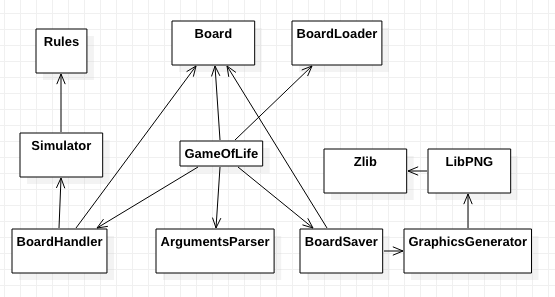
\includegraphics[width=13cm]{diagram_modolow.png}
\end{figure}	

\subsection{GameOfLife}
Główny moduł kontrolujący przepływ sterowania i danych między pozostałymi modułami.

\subsubsection{Funkcje}
\texttt{int main(int argc, char** args)} -- Punkt startowy programu. Z niej wywoływane będą kolejne funkcje. Przyjmować będzie 2 argumenty -- argumenty wsadowe programu:\\\\
	 \hspace*{10mm}\texttt{int argc} -- ilość argumentów,\\\\
	 \hspace*{10mm}\texttt{char** args} -- tablica napisów -- faktycznych argumentów wywołania	 \hspace*{34mm} programu.\\

\subsection{ArgumentsParser}
Moduł odpowiadający za interpretacje podanych wsadowo argumentów programu, konwersji ich oraz zapisu do utworzonej w tym celu struktury.

\subsubsection{Funkcje}
\texttt{params parseArgs(int argc, char** argv)} -- będzie przetwarzać argumenty wsadowe programu podane w postaci flag na strukturę zawierającą ustawienia symulacji. Przyjmować będzie 2 argumenty -- argumenty wsadowe programu:\\\\
	 \hspace*{10mm}\texttt{int argc} -- ilość argumentów,\\\\
	 \hspace*{10mm}\texttt{char** args} -- tablica napisów, będących faktycznymi argumentami wy-\hspace*{10mm}wołania programu.\\
\\
Zwracać będzie strukturę zawierająca ustawienia symulacji.

\subsection{BoardSaver}
Moduł odpowiadający za obsługę zapisu wyników działania programu w zależności od argumentów.

\subsubsection{Funkcje}
\texttt{void save(board* b, config c)} -- będzie uruchamiać konkretne funkcję zapisujące w zależności od podanych flag. Jako argument będzie przyjmować wskaźnik na strukturę zawierającą opis planszy:\\\\
	 \hspace*{10mm}\texttt{board* b} -- wskaźnik na strukturę zawierającą opis planszy,\\\\
\\
\texttt{void saveTxt(board* b, config c)} -- Będzie zapisywać dany stan planszy w pliku tekstowym, mogącym w przyszłości służyć za plik wejściowy. Jako argument będzie przyjmować wskaźnik na strukturę zawierającą opis planszy:\\\\
	 \hspace*{10mm}\texttt{board* b} -- wskaźnik na strukturę zawierającą opis planszy,\\\\
\\

\subsection{GraphicsGenerator}
Moduł odpowiadający za obsługę zapisu wyników działania programu w zależności od argumentów.

\subsubsection{Funkcje}
\texttt{void savePng(char* data, config c)} -- będzie generować plik .png będący reprezentacją planszy :\\\\
	 \hspace*{10mm}\texttt{char* data} -- dane opisujące planszę, potrzebne do generacji pliku .png,\\\\
	  \hspace*{10mm}\texttt{config c} -- struktura zawierająca parametry pliku wyjściowego.\\\\
\\
\texttt{void saveGif(char* data, config c)} -- będzie generować plik .gif będący reprezentacją planszy :\\\\
	 \hspace*{10mm}\texttt{char* data} -- dane opisujące planszę, potrzebne do generacji pliku .gif,\\\\
	  \hspace*{10mm}\texttt{config c} -- struktura zawierająca parametry pliku wyjściowego.\\\\
\\





\subsubsection{Struktury}
Struktura zawierająca ustawienia symulacji: \\\\
\texttt{typedef struct\{\\
	 \hspace*{10mm}int help;\\
	 \hspace*{10mm}char* file;\\
	 \hspace*{10mm}char* output\_dest;\\
	 \hspace*{10mm}char* type;\\
	 \hspace*{10mm}int number\_of\_generations;\\
	 \hspace*{10mm}int step;\\
	 \hspace*{10mm}int delay;\\
\}config;\\}
\\
\texttt{help} -- informuje o tym czy ma być wyświetlana pomoc,\\
\texttt{file} -- informuje o tym jaka jest ścieżka do pliku wejściowego,\\
\texttt{output\_dest} --  informuje o tym jaka jest ścieżka dla pliku/plików wyjściowych,\\
\texttt{type} -- informuje o tym jaki jest typ zwracanych wyników,\\
\texttt{number\_o\_generations} -- informuje o tym ile pokoleń komórek zostanie wygenerowane,\\
\texttt{step} -- informuje o tym co ile pokoleń zapisywane będą dane wyjściowe,\\
\texttt{delay} -- informuje w jakich odstępach czasu mają się wyświetlać kolejne generacje komórek.\\

\subsection{BoardHandler}
Moduł definiujący strukturę planszy -- \textit{Board} oraz podstawowe funkcje związane z tą strukturą.

\subsubsection{Struktury}

Typ wyliczeniowy zawierający możliwe stany pojedynczej komórki. \\
\texttt{typedef enum\{\\
	 \hspace*{10mm}DEAD = 0,\\
	 \hspace*{10mm}ALIVE = 1\\
\}CellState;\\} \\
\texttt{DEAD} -- Komórka jest martwa \\
\texttt{ALIVE} -- Komórka jest żywa

\vspace*{10mm}

\noindent{}Struktura przechowująca stan pojedynczego pokolenia. \\
\texttt{typedef struct\{\\
	 \hspace*{10mm}int sizeX;\\
	 \hspace*{10mm}int sizeY;\\
	 \hspace*{10mm}CellState *cells;\\
\}Board;\\} \\
\texttt{sizeX} -- Szerokość planszy \\
\texttt{sizeY} -- Wysokość planszy \\
\texttt{cells} -- Tablica zawierająca stany wszystkich komórek

\subsubsection{Funkcje}

\texttt{Board* createRandomBoard(int x, int y)} -- Tworzy planszę o podanej wielkości z komórkami o losowych stanach. Zwracany jest wskaźnik na nowy obiekt \texttt{Board} utworzony na stercie. \\
\hspace*{10mm}\texttt{int x} -- szerokość planszy\\
\hspace*{10mm}\texttt{int y} -- wysokość planszy\\

\vspace*{8mm}
\noindent{}\texttt{void disposeBoard(Board *board)} -- Zwalnia dynamicznie alokowane pola struktury \texttt{Board}. Powinna zostać wywołana przed zwolnieniem dowolnej zmiennej typu \texttt{Board}. Po zastosowaniu tej metody zmienna wskazana przez argument \texttt{board} nie nadaje się już do użytku. \\ \\
\hspace*{10mm}\texttt{Board *board} -- Adres planszy, która będzie zwalniana\\

\vspace*{8mm}
\noindent{}\texttt{char* boardToString(Board *board)} -- Generuje ciąg znaków reprezentujący stan wskazanej planszy. Zwrócony napis należy po wykorzystaniu zwolnić. \\ \\
\hspace*{10mm}\texttt{Board *board} -- Adres planszy, której reprezentacja ma zostać wygenerowana\\

\vspace*{8mm}
\noindent{}\texttt{char* serializeBoard(Board *board)} -- Generuje ciąg znaków reprezentujący wskazaną strukturę \texttt{Board}. Zwrócony napis zawiera wszystkie niezbędne informacje do rekonstrukcji struktury na jego podstawie. Zwrócony napis należy po wykorzystaniu zwolnić. \\ \\
\hspace*{10mm}\texttt{Board *board} -- Adres planszy, której reprezentacja ma zostać wygenerowana


\subsection{Simulator}
Moduł odpowiadający za przeprowadzenie właściwej symulacji zgodnie z regułami gry w życie.

\subsubsection{Funkcje}
\texttt{board* simulate(board* b, params p)} -- będzie przeprowadzać symulacje całej gry w życie:\\\\
	 \hspace*{10mm}\texttt{board* b} -- wskaźnik na strukturę zawierającą stan planszy,\\
	 \hspace*{10mm}\texttt{params p} -- struktura zawierająca ustawienia symulacji.\\
\\
Zwracać będzie strukturę zawierająca końcowy stan planszy.\\\\
\\
\texttt{board nextGen(board* b)} -- będzie generować planszę odpowiadającą następnemu pokoleniu komórek. Jako argument będzie przyjmować:\\\\
	 \hspace*{10mm}\texttt{board* b} -- wskaźnik na strukturę zawierającą stan planszy,\\
\\
Zwracać będzie wskaźnik na strukturę zawierająca stan planszy w następnym pokoleniu.

\subsection{Loader}
Moduł odpowiedzialny za wczytanie planszy początkowej z pliku tekstowego i zapisanie jej do struktury.

\subsubsection{Funkcje}
\texttt{board* load(char* path)} -- będzie przetwarzać plik wejściowy i zapisywać go do struktury. Jako argument będzie przyjmować:\\\\
	 \hspace*{10mm}\texttt{char* path} -- ścieżka do pliku wejściowego,\\
\\
Zwracać będzie wskaźnik na strukturę opisującą początkowy stan planszy.\\\\
\\
\texttt{int* getSize(char* path)} -- będzie wczytywać rozmiar planszy zapisanej w pliku wejściowym:\\\\ %Nie wiem czy to jest potrzebne
	 \hspace*{10mm}\texttt{char* path} -- ścieżka do pliku wejściowego,\\
\\
Zwracać będzie dwuelementowy wektor zawierający rozmiary planszy początkowej.

\section{Kompilacja}
W celu automatyzacji procesu kompilacji wykorzystane zostanie narzędzie \textit{makefile}. Umożliwi ono przygotowanie scenariuszy kompilacji na różne środowiska.

\subsection{Środowisko testowe}
Środowisko to ma na celu optymalizację prędkości kompilacji i umieszczenie symboli pozwalających na sprawne debugowanie kodu w plikach wynikowych. Przy kompilacji testowej zostanie zdefiniowana stała \texttt{DEBUG}. Dzięki temu wykorzystując mechanizm kompilacji warunkowej możliwe będzie wyświetlenie dodatkowych informacji o działaniu programu w trybie testowym.

\paragraph{Lista flag:}
\begin{itemize}
	\item \texttt{-O0} -- Optymalizacja czasu kompilacji
	\item \texttt{-std=c11} -- Ustawienie standardu języka C
	\item \texttt{-Wall} -- Wypisywanie wszystkich ostrzeżeń
	\item \texttt{-g3} -- Umieszczenie pełnych symboli do debugowania
	\item \texttt{-D DEBUG} -- Ustawienie stałej preprocesora o nazwie \texttt{DEBUG}
\end{itemize}

\subsection{Środowisko produkcyjne}
Środowisko to ma na celu optymalizację zasobów wykorzystywanych przez program w trakcie działania.

\paragraph{Lista flag:}
\begin{itemize}
	\item \texttt{-Ofast} -- Optymalizacja zasobów kosztem czasu kompilacji
	\item \texttt{-std=c11} -- Ustawienie standardu języka C
	\item \texttt{-g0} -- Nie umieszczenie symboli do debugowania
\end{itemize}

\section{Testy}
Poprawność działania funkcji zawartych w modułach programu będzie testowana przy pomocy testów jednostkowych. W celu organizacji oraz uspójnienia testów zostanie wykorzystany framework \textbf{CUnit}.

\subsection{Stuktóra testów}
Testy zostaną podzielone na zestawy. Każdy zestaw będzie grupował testy dotyczące danej części projektu (najczęściej modułu, ale koniecznie). Dzięki podziałowi testów łatwiej będzie zidentyfikować kod wywołujący problemy.

\subsection{Planowane testy}
%TODO: Opisać jakie testy chcemy robić

\paragraph{Test zamiany planszy na ciąg znaków} będzie polegał na ręcznym utworzeniu struktury planszy o konkretym stanie komórek. Następnie zostanie utworzona reprezentacja tekstowa planszy przy pomocy funkcji \\ \texttt{char* boardToString(Board *board)}. Powstały w ten sposób tekst zostanie porównany z ręcznie wpisaną spodziewaną wartością.

\paragraph{Test parsowania planszy} będzie polegał na utworzeniu tymczasowego pliku zawierającego tekst w formacie pliku przechowującego stan planszy. Następnie zostanie wywołana funkcja \texttt{board* load(char* path)}. Kolejnym krokiem będzie sprawdzenie czy szerokość, długość i wartości komórek wczytanej planszy są takie jak spodziewane. Jeśli te warunki zostaną spełnione wynik testu będzie pozytywny. Pod koniec testu usunięty zostanie plik tymczasowy.

%TODO: Napisać jaka funkcja jest wywoływana z modułu zasad
\paragraph{Test reguł} będzie weryfikował czy zasady generacji komórek następnego pokolenia przeważają poprawnie otrzymany obszar. W jego trakcie do modułu zasad zostanie przekazany obszar hipotetycznej planszy. Wynik realizacji reguł generacji następnego pokolenia na danym obszarze zostanie porównany ze spodziewanym obszarem. Jeśli wszystkie komórki będą miały identyczne stany test zakończy się pozytywnie.

\paragraph{Test symulacji} ma za zadanie zweryfikować proces wytworzenia całego nowego pokolenia na podstawie poprzedniego. W tym celu zostanie utworzona plansza o znanym stanie komórek. Będzie ona przekazana funkcji \texttt{board simulate\\(board b, params p)}. Nowa plansza powstała w wyniku działania funkcji symulującej zostanie porównana ze spodziewanym stanem planszy. Jeśli jakakolwiek z komórek będzie różna między wynikiem symulacji a wartością spodziewaną test zakończy się niepowodzeniem.

\section{Test wczytania argumentów wsadowych} będzie polegał na utworzeniu napisu reprezentującego flagi podane przez użytkownika. Następnie zostanie wywołana funkcja \texttt{params parseArgs(int argc, char** argv)}. Zwrócona struktura ustawień zostanie porównana pole po polu ze spodziewanym wynikiem. Jeśli wszystkie pola spodziewanych ustawień będą takie same jak tych powstały w wyniku parsowania flag programu test zakończy się powodzeniem.

\section{Biblioteki zewnętrzne}
Program będzie korzystał z bibliotek nie będących częścią standardu języka C. Umożliw to dostarczenie szerszej funkcjonalności.

\subsection{zlib.h}
Biblioteka zawierająca darmową implementację algorytmów kompresji i dekompresji \textit{deflate}. Jest ona wykorzystywana wewnętrznie przez bibliotekę \texttt{libpng.h}.

\subsection{libpng.h}
Biblioteka ta umożliwia tworzenie oraz odczytywanie plików graficznych takich jak \textit{png} czy \textit{gif}.

\subsection{cunit.h}
Jest to framework służący do tworzenia i uruchamiania testów jednostkowych. Zostanie wykorzystany do uspójnienia procesu testowania modłów programu.

\end{document}
